\documentclass{article}\usepackage[]{graphicx}\usepackage[]{color}
%% maxwidth is the original width if it is less than linewidth
%% otherwise use linewidth (to make sure the graphics do not exceed the margin)
\makeatletter
\def\maxwidth{ %
  \ifdim\Gin@nat@width>\linewidth
    \linewidth
  \else
    \Gin@nat@width
  \fi
}
\makeatother

\definecolor{fgcolor}{rgb}{0.345, 0.345, 0.345}
\newcommand{\hlnum}[1]{\textcolor[rgb]{0.686,0.059,0.569}{#1}}%
\newcommand{\hlstr}[1]{\textcolor[rgb]{0.192,0.494,0.8}{#1}}%
\newcommand{\hlcom}[1]{\textcolor[rgb]{0.678,0.584,0.686}{\textit{#1}}}%
\newcommand{\hlopt}[1]{\textcolor[rgb]{0,0,0}{#1}}%
\newcommand{\hlstd}[1]{\textcolor[rgb]{0.345,0.345,0.345}{#1}}%
\newcommand{\hlkwa}[1]{\textcolor[rgb]{0.161,0.373,0.58}{\textbf{#1}}}%
\newcommand{\hlkwb}[1]{\textcolor[rgb]{0.69,0.353,0.396}{#1}}%
\newcommand{\hlkwc}[1]{\textcolor[rgb]{0.333,0.667,0.333}{#1}}%
\newcommand{\hlkwd}[1]{\textcolor[rgb]{0.737,0.353,0.396}{\textbf{#1}}}%

\usepackage{framed}
\makeatletter
\newenvironment{kframe}{%
 \def\at@end@of@kframe{}%
 \ifinner\ifhmode%
  \def\at@end@of@kframe{\end{minipage}}%
  \begin{minipage}{\columnwidth}%
 \fi\fi%
 \def\FrameCommand##1{\hskip\@totalleftmargin \hskip-\fboxsep
 \colorbox{shadecolor}{##1}\hskip-\fboxsep
     % There is no \\@totalrightmargin, so:
     \hskip-\linewidth \hskip-\@totalleftmargin \hskip\columnwidth}%
 \MakeFramed {\advance\hsize-\width
   \@totalleftmargin\z@ \linewidth\hsize
   \@setminipage}}%
 {\par\unskip\endMakeFramed%
 \at@end@of@kframe}
\makeatother

\definecolor{shadecolor}{rgb}{.97, .97, .97}
\definecolor{messagecolor}{rgb}{0, 0, 0}
\definecolor{warningcolor}{rgb}{1, 0, 1}
\definecolor{errorcolor}{rgb}{1, 0, 0}
\newenvironment{knitrout}{}{} % an empty environment to be redefined in TeX

\usepackage{alltt}
\usepackage{amsmath,amsfonts,bm,fullpage}
\usepackage{natbib}
\newcommand{\ProjMean}{{\widehat{\bm S}_{2}}}
\IfFileExists{upquote.sty}{\usepackage{upquote}}{}
\begin{document}




\begin{center}
\Large{\bf Outlier Detection for Circular and Spherical Data}
\end{center}
\normalsize
In this document I summarize the work done for outlier detection for circular, spherical and related data types

\section{Circular Data}

In \cite{collett1980}, four statistics to identify outliers in circular data are defined.  Only the von Mises distribution on the circle is considered in the simulation study, but three of the statistics are general and could be applied to any circular distribution. 

The $L$-statistic is the likelihood ratio test statistic that tests the null hypothesis that all observations are from a single von Mises($\mu,\kappa$) versus the alternative that one observation comes from a von Mises distribution with a different mean direction.  This is sometimes called the location-slippage alternative hypothesis.  The test-statistic in the context of the von Mises distribution for the observation $\theta_k$ is
\[
L=(R_k+1)\hat{\kappa}_k-\hat{\kappa}R-n\log\left[\frac{I_0(\hat{\kappa}_k)}{I_0(\hat{\kappa})}\right]
\]
where $R_k$ and $\hat\kappa_k$ are the estimated mean resultant lengths and concentration parameter with $\theta_k$ removed and $I_0(x)$ is the modified Bessel function of the first kind with order zero.

The $C$-Statistic is more general.  It is interpreted as the relative increase in the sample mean resultant length after omitting the queried value.  It is given by
\[
C=\text{max}_i\left\{\frac{\bar{R}_i-\bar{R}}{\bar{R}}\right\}=\frac{R_k-R}{R}
\]
where $\bar{R}$ is the sample mean resultant length and $\bar{R}_i$ is the mean resultant length with the $i$th observation removed.  

The $D$-statistic is the ratio of the arcs on either side of the observation.  That is, let $\theta_{(i)}$ denote the $i$th ordered observation and define
\[
T_i=\theta_{(i+1)}-\theta_{(i)}\hspace{1em}\text{ and }\hspace{1em}T_n=2\pi-\theta_{(n)}+\theta_{(i)}.
\]
 Also set $T_{0}=T_{n}$ then for $i=1,\dots,n$, $D_i=T_i/T_{i-1}$ is the ratio of the arc-lengths on either side of the $i$th observation.  Finally let $\theta_k$ be the observation that visually appears to be an outlier and define $D=\text{min}(D_k,D_{k}^{-1})$ then $D\in(0,1)$ and is unambiguous.

\begin{knitrout}
\definecolor{shadecolor}{rgb}{0.969, 0.969, 0.969}\color{fgcolor}

{\centering 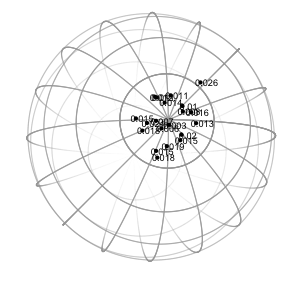
\includegraphics[width=.4\linewidth]{Figure/dstat} 

}



\end{knitrout}






Finally, the $M$-statistic was originally suggested by Mardia (1975) \cite{mardia1975} and is similar in spirit to the $C$-statistic, namely
\[
M=\min_i\left(\frac{n-1-R_i}{n-R}\right)
\]
where $R$ is mean resultant length based on the entire sample of size $n$ and $R_i$ is the mean resultant length after the $i$th observation is deleted.  To put this on the same scale as the other statistics discussed in \cite{collett1980} consider $1-M$.

In a simulation study they determine the $C$ and $D$ statistics are the best choices.  Because $D$ is easier to compute it comes the most highly recommended.

According to Mardia et al. (2009) \cite{mardia2009},  Best \& Fisher (1986) \cite{best1986} and Bagchi \& Guttman \cite{bagchi1990} consider other ways to identify outliers but I can't get a hold of either of these articles to read.

\section{Spherical Data}

Fisher, Lewis \& Willcox (1981) \cite{fisher1981} extend the statistics of \cite{collett1980} to spherical data and also add a few of their own.  Several outliers in a single sample are also considered.  They focus on Fisher's distribution on the sphere.

The spherical analog of Collett's $C$-statistic is
\[
C_n=\frac{\bar{R}_n^{(i)}-\bar{R}_n}{\bar{R}_n}.
\]

Using the approximations coth$(\kappa)\approx 1$ and $\log(\text{sinh}\kappa)\approx\kappa-\log 2$ the spherical analogs of Collett's $M$ (and for $\kappa>2.5$ Collett's $L$) is 
\[
E_n=(n-2)\frac{1+R_{n-1}^{(i)}-R_n}{n-1-R_{n-1}^{(i)}}.
\]
$E_n$ is based on a generalised likelihood-ratio test statistic testing the alternative location-slippage hypothesis.

Alternative, one can test the alternative hypothesis that the mean directions are the same, but the concentration parameters are different.  This leads to the generalised likelihood-ratio test-statistic
\[
D_n=(n-1)f(\bar{R}_{n-1}^{(i)})+f(\bar{R}_1^{(i)})-nf(\bar{R}_n)
\]
where $f(\bar{r})=\log\hat\kappa(\bar{r})+(\bar{r}-1)\hat\kappa(\bar{r})$ and $\kappa(\bar{r})$ is the concentration parameter estiamte based on the sample mean resultant length $\bar{r}$.

Let $l_i$, $m_i$ and $n_i$ be the direction cosines for $(\theta_i,\phi_i)$, $1\leq i\leq n$ and let $l_i'$, $m_i'$ and $n_i'$ be the direction cosines after they've been centered around a pole.  Define $\theta_i'=\cos^{-1}(n_i')$ and $c_i=1-n_i'$ then order them $\theat_{(i)}'$ and $c_{(i)}$.  The gap test for an outlying observation can be based on
\[
G_n=\frac{\pi-\theta_{(n)}'}{\theta_{(n)}'-\theta_{(n-1)}'}.
\]

The test statistic Ea 1 of Barnett and Lewis ()
\bibliographystyle{plain}
\bibliography{RobustRefs}

\end{document}
